\documentclass[12pt]{report}
\usepackage{inconsolata}
\usepackage{lmodern}
\usepackage[utf8]{inputenc}
\usepackage{listings}
\usepackage{graphicx}
\usepackage{caption}
\usepackage{subcaption}
\usepackage[czech]{babel}
\usepackage{titlesec}
\usepackage{lipsum}
\graphicspath{{Images/}}
\usepackage[style=numeric, sorting=none]{biblatex}
\addbibresource{Zdroj.bib}
\usepackage{ragged2e}
\linespread{1.5}
\setlength{\hsize}{0.9\hsize}
\usepackage{wrapfig}
\usepackage{tgtermes}
\usepackage{parskip}
\usepackage{titlesec}
\usepackage[T1]{fontenc}
\usepackage{inconsolata}
\usepackage{appendix}
\usepackage[colorlinks=true, allcolors=black]{hyperref}
\usepackage{amsmath}
\usepackage{amsfonts}
\usepackage{amssymb}
\usepackage{bm}
\usepackage{tabto}
\usepackage{setspace}
\usepackage[a4paper, left = 3.5cm, top = 2.5cm, bottom = 2.5cm, right = 2.5cm]{geometry}
\usepackage{url}
\usepackage{xcolor}
\usepackage{float}
\usepackage{csquotes}
\addbibresource{Zdroj.bib}

% color def
\usepackage{color}
\definecolor{editorGreen}{rgb}{0.18,0.80,0.18}
\definecolor{editorOcher}{rgb}{0.99,0.48,0.13}
\definecolor{gray}{rgb}{0.95,0.95,0.98}
\definecolor{darkred}{rgb}{0.6,0.0,0.0}
\definecolor{darkgreen}{rgb}{0,0.50,0}
\definecolor{lightblue}{rgb}{0.0,0.42,0.91}
\definecolor{orange}{rgb}{0.99,0.48,0.13}
\definecolor{grass}{rgb}{0.18,0.80,0.18}
\definecolor{pink}{rgb}{0.97,0.15,0.45}
% General Setting of listings
\lstset{
  aboveskip=1em,
  breaklines=true,
  abovecaptionskip=-6pt,
  captionpos=b,
  escapeinside={\%*}{*)},
  frame=single,
  numbers=left,
  numbersep=15pt,
  numberstyle=\tiny,
}
% 0. Basic Color Theme
\lstdefinestyle{colored}{ %
  basicstyle=\ttfamily,
  backgroundcolor=\color{white},
  commentstyle=\color{green}\itshape,
  keywordstyle=\color{blue}\bfseries\itshape,
  stringstyle=\color{red},
}
% 1. General Python Keywords List
\lstdefinelanguage{PythonPlus}[]{Python}{
  morekeywords=[1]{,as,assert,nonlocal,with,yield,self,True,False,None,} % Python builtin
  morekeywords=[2]{,__init__,__add__,__mul__,__div__,__sub__,__call__,__getitem__,__setitem__,__eq__,__ne__,__nonzero__,__rmul__,__radd__,__repr__,__str__,__get__,__truediv__,__pow__,__name__,__future__,__all__,}, % magic methods
  morekeywords=[3]{,object,type,isinstance,copy,deepcopy,zip,enumerate,reversed,list,set,len,dict,tuple,range,xrange,append,execfile,real,imag,reduce,str,repr,}, % common functions
  morekeywords=[4]{,Exception,NameError,IndexError,SyntaxError,TypeError,ValueError,OverflowError,ZeroDivisionError,}, % errors
  morekeywords=[5]{,ode,fsolve,sqrt,exp,sin,cos,arctan,arctan2,arccos,pi, array,norm,solve,dot,arange,isscalar,max,sum,flatten,shape,reshape,find,any,all,abs,plot,linspace,legend,quad,polyval,polyfit,hstack,concatenate,vstack,column_stack,empty,zeros,ones,rand,vander,grid,pcolor,eig,eigs,eigvals,svd,qr,tan,det,logspace,roll,min,mean,cumsum,cumprod,diff,vectorize,lstsq,cla,eye,xlabel,ylabel,squeeze,}, % numpy / math
}
% 2. New Language based on Python
\lstdefinelanguage{PyBrIM}[]{PythonPlus}{
  emph={d,E,a,Fc28,Fy,Fu,D,des,supplier,Material,Rectangle,PyElmt},
}
% 3. Extended theme
\lstdefinestyle{python}{
  basicstyle=\tiny\ttfamily,
  backgroundcolor=\color{gray},
  commentstyle=\color{darkgreen}\slshape,
  keywordstyle=\color{blue}\bfseries\itshape,
  keywordstyle=[2]\color{blue}\bfseries,
  keywordstyle=[3]\color{grass},
  keywordstyle=[4]\color{red},
  keywordstyle=[5]\color{orange},
  stringstyle=\color{darkred},
  emphstyle=\color{pink}\underbar,
}

\hyphenpenalty=10000\exhyphenpenalty=10000


\begin{document}
\titleformat{\chapter}
  {\normalfont\LARGE\bfseries}{\thechapter}{1em}{}
\titlespacing*{\chapter}{0pt}{3.5ex plus 1ex minus .2ex}{2.3ex plus .2ex}

\renewcommand{\figurename}{Obr.}
\renewcommand{\lstlistingname}{Ukázka kódu}
\spacing{1.5}
\begin{titlepage}

\begin{center}

    {\LARGE \textbf{ Gymnázium, Praha 6, Arabská 14}}

    \vspace{0.5cm}

    {\Large Obor programování}

    \vspace{1cm}
    
    {\Huge \textbf{Ročníková práce}}

    \vspace{1cm}

    \begin{figure*}[h]
        \centering
        
\includegraphics[width=0.75\linewidth]{Images/Logo.png}
    \end{figure*}

    \vspace{1cm}

    {\Large Ivan Merkulov}

    \vspace{1cm}
    
    {\Huge \textbf{Snake AI}}

    \vspace{2cm}
    
    {\Large Duben 2025}
    
\end{center}

\end{titlepage}
\begin{titlepage}

\vspace{1.5cm}

\begin{center}
    {\LARGE \textbf{ Gymnázium, Praha 6, Arabská 14}}

    \vspace{1.0cm}

    {\Large Arabská 14, Praha 6, 160 00}

    \vspace{3.5cm}
 
    {\Huge \textbf{Ročníková práce}}
\end{center}

\vspace{6.0cm}

\textbf{Předmět:} {\large Programování}

\textbf{Téma:} {\large Snake AI}

\vspace{1.5cm}

\textbf{Školní rok:}  {\large2024/2025 }


\textbf{Autor:} {\large Ivan Merkulov}


\textbf{Třída:} {\large 4.E}


\textbf{Vedoucí práce:} {\large Mgr. Jan Lána}


\textbf{Třídní učitel:} {\large Mgr. Blanka Hniličková}

\end{titlepage}


\thispagestyle{empty}
\newpage
\newpage

\thispagestyle{empty}
\vspace*{\fill}

Prohlašuji, že jsem jediným autorem tohoto projektu, všechny citace jsou řádně označené a všechna použitá literatura a další zdroje jsou v práci uvedené. Tímto dle zákona 121/2000 Sb. (tzv. Autorský zákon) ve znění pozdějších předpisů uděluji bezúplatně škole Gymnázium, Praha 6, Arabská 14 oprávnění k výkonu práva na rozmnožování díla (§ 13) a práva na sdělování díla veřejnosti (§ 18) na dobu časově neomezenou a bez omezení územního rozsahu.

\vspace{2cm}

V Praze dne 7. dubna 2025 \hspace{7cm}\line(1,0){3cm}
\thispagestyle{empty}
\setcounter{page}{0}

\section*{Anotace}
Tato práce se zabývá vývojem a implementací hry Snake, a umělé inteligence ovládající hada tak, že zaplní celé hrací pole, aniž by došlo ke kolizi. Hlavním cílem je nalezení optimální cesty k jablku a minimalizace rizika srážky prostřednictvím různých algoritmů. V rámci práce budou analyzovány a porovnány různé metody plánování pohybu, jako je A* algoritmus a algoritmy pro hledání Hamiltonovské kružnice. Výsledkem práce bude nejen funkční implementace hry, ale také vyhodnocení efektivity jednotlivých přístupů.

\section*{Abstract}
This work focuses on developing and implementing a Snake game in which the snake plays autonomously and completes the game by filling the entire playing field without colliding. The main objective is to find an optimal path to the apple while minimizing the risk of collision using various algorithms. The work analyzes and compares different pathfinding methods, such as the A* algorithm and algorithms for finding Hamiltonian cycles. The result of this work is a functional implementation of the game together with an evaluation of the efficiency of different approaches.

\section*{Anmerkung}
Diese Arbeit befasst sich mit der Entwicklung und Implementierung eines Snake-Spiels, in dem die Schlange autonom spielt und das Spiel beendet, indem sie das gesamte Spielfeld füllt, ohne mit sich selbst zu kollidieren. Das Hauptziel ist es, einen optimalen Weg zum Apfel zu finden und gleichzeitig das Kollisionsrisiko durch verschiedene Algorithmen zu minimieren. In dieser Arbeit werden verschiedene Methoden zur Pfadsuche analysiert und verglichen, darunter der A*-Algorithmus und Algorithmen zur Suche nach Hamiltonschen Zyklen. Das Ergebnis dieser Arbeit wird nicht nur eine funktionale Implementierung des Spiels sein, sondern auch eine Bewertung der Effizienz verschiedener Ansätze.
\newpage


\include{Kapitoly/Zadani}

\renewcommand{\contentsname}{Obsah}
\tableofcontents

\chapter{Úvod}

Hra Snake patří mezi klasické počítačové hry, které si získaly popularitu díky své jednodu-\\chosti, ale zároveň rostoucí obtížnosti. Tradičně je had ovládán hráčem, avšak v této práci se zaměřím na vytvoření autonomní verze hry, kde had sám dokáže dohrát hru až do zaplnění celého hracího pole. Aby se had mohl efektivně navigovat herním prostředím, bude využívat algoritmy pro hledání nejoptimálnější cesty k jablku a zároveň se vyhýbat kolizím. 

Mezi hlavní metody patří \(A*\) algoritmus, který je široce používán pro hledání nejkratších cest, a algoritmy zaměřené na hledání Hamiltonovských kružnic, které umožňují průchod všemi poli bez opakované návštěvy stejného místa. V práci se budu věnovat nejen implemen-\\taci samotné hry, ale také porovnání různých přístupů z hlediska jejich efektivity, výpočetní náročnosti a schopnosti hada úspěšně dokončit hru.

\section{Hra Snake}

Hra Snake je jednoduchá arkádová hra, ve které hráč ovládá hada pohybujícího se po hracím poli. Cílem hry je sbírat jablka, která se náhodně objevují na hrací ploše. Po sebrání jablka se had vždy prodlouží o jedno políčko. Hra končí v okamžiku, kdy had narazí do stěny nebo do svého vlastního těla.

Hráč ovládá hada pomocí směrových kláves, čímž mění směr jeho pohybu nahoru, dolů, doleva nebo doprava. Had se pohybuje konstantní rychlostí, a jakmile hráč změní směr, had okamžitě reaguje a pokračuje v pohybu daným směrem. Není možné se otočit o 180 stupňů, což znamená, že had nemůže jít zpět po své vlastní trase.

\begin{figure}[H]
    \centering
    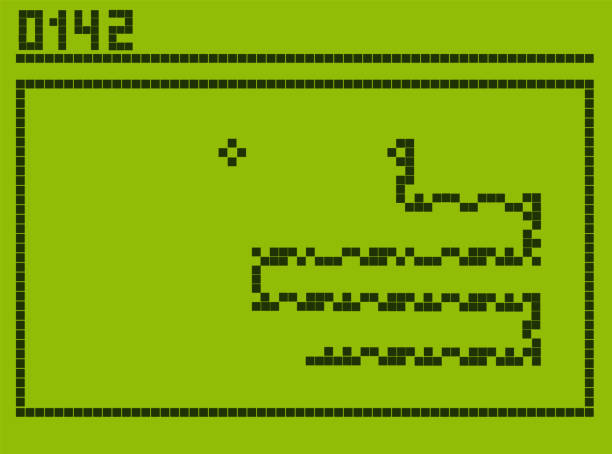
\includegraphics[width=0.5\linewidth]{Images/SnakeGame.jpg}
    \caption[Dostupné z: \url{https://www.istockphoto.com/cs/search/2/image-film?phrase=snake+game}]{Hra Snake}
    \label{fig:SnakeGame}
\end{figure}

V této práci se budu zabývat verzí hry, ve které se had pohybuje v omezeném prostoru s pevnými hranicemi. Hrací pole má obdélníkový tvar a je ohraničeno zdí, která tvoří pevnou bariéru. Jakmile had narazí do této zdi, hra končí. Toto omezení vyžaduje, aby had efektivně plánoval své pohyby a předcházel situacím, kdy by se ocitl v pasti. V této variantě hry neexistuje možnost průchodu skrz okraje obrazovky, což činí navigaci složitější a nutí hada efektivně optimalizovat svůj pohyb.

\section{Zadání práce}
Cílem mé práce je pokusit se o napsání hry Snake, ve které Snake sám dohraje hru (to znamená, že zaplní celý prostor hracího pole, aniž by se zabil). Snake se bude snažit najít optimální cestu k jablku a přitom se bude vyhýbat kolizím. Pomocí různých algoritmů se pokusím o to, aby Snake dokázal najít jablko co nejoptimálněji a pokud možno nejlépe dohrál hru. V práci se budu snažit využít algoritmy na hledání Hamiltonovské kružnice a algoritmus A*. Součástí práce bude porovnání výsledků použitých algoritmů.

\section{Použité technologie}
Práce je napsaná v programovacím jazyce Python, s využitím knihovny Pygame na vykres-\\lování herního pole hry Snake.

\section{Analýza problému a řešení}

Pro úspěšnou implementaci autonomní verze hry Snake je nutné vyřešit několik klíčových problémů. Jedním z hlavních aspektů je reprezentace herního pole a samotného hada. Hrací plocha je modelována jako dvourozměrná mřížka, kde každá buňka může být prázdná, obsahovat tělo hada nebo jablko. Had je reprezentován jako seznam souřadnic jeho těla, kde první prvek odpovídá hlavě hada.

Aby bylo možné efektivně plánovat pohyb hada, problém navigace lze chápat jako hledání cesty v grafu, kde uzly představují jednotlivé buňky hracího pole a hrany odpovídají možným tahům. Hledání nejkratší cesty probíhá mezi hlavou hada a jablkem, což snižuje výpočetní náročnost oproti sledování celého těla. Hlavní výzvou je nejen nalezení efektivní trasy k jablku, ale také zajištění toho, aby had nezablokoval svůj vlastní pohyb a měl dostatečný prostor pro další růst. Kromě toho musí být strategie hada navržena tak, aby umožnila zaplnění celé hrací plochy, tedy úspěšné dokončení hry.
\chapter{Implementace grafu}\label{Implementace grafu}
Hra Snake probíhá na čtvercovém hracím poli, kde se had pohybuje a snaží se sníst jablka, která se na něm objevují. Had se pohybuje postupně po jednotlivých políčkách, přičemž musí optimalizovat svou trasu tak, aby dosáhl jablka co nejefektivněji a zároveň se neuvěznil ve vlastní stopě. Abychom mohli efektivně řídit jeho pohyb a hledat nejkratší cesty, můžeme tento problém převést na graf. 

Hrací pole obsahuje \(n \times n\) políček, kde \(n\) je počet políček na jedné straně. Takové hrací pole dokážeme jednoduše reprezentovat jako čtvercový graf, což je graf, jehož vrcholy jsou uspořádány do pravidelné pravoúhlé mřížky o \(n^2\) vrcholech. Každý vrchol bude reprezen-\\tovat jedno políčko v hracím poli. Hrany grafu pak reprezentují možné pohyby hada mezi sousedními políčky. Každý vrchol má různý počet hran v závislosti na své poloze v mřížce. Do vrcholů reprezentující rohová políčka povedou dvě hrany. Uzly, které představují políčka na okraji hracího pole, budou napojeny třemi hranami a do vrcholů, které jsou uprostřed, vedou čtyři hrany. 

Tento graf lze reprezentovat dvěma způsoby: staticky, kdy se celý graf předem vygeneruje a uloží, nebo dynamicky, kdy se vrcholy a hrany vytvářejí pouze podle potřeby.

\section{Statická reprezentace}\label{Staticky}
V statické reprezentaci grafu si vygenerujeme najednou graf pro celé hrací pole a celý graf si uložíme do paměti. Tento graf nebudeme následně během hry nijak měnit. Pokud chceme provést změny v grafu, musíme celý graf smazat a vygenerovat nový graf, reflektují-\\ cí všechny požadované změny. 

Taková reprezentace je výhodná, pokud graf využíváme jako reprezentaci nějaké situace, která se nemění, tedy že se nemění graf, se kterým pracujeme. Např., když potřebujeme najít nejkratší cestu na mapách, stejnou mapu v tomto případě lze využít i opakovaně. Nejprve najdeme například nejkratší cestu domu a pokud budeme sledovat nalezenou trasu, cesta se v průběhu pohybu měnit nebude. Následně můžeme využít stejného grafu (mapy), abychom našli cestu z domova do školy, ze školy na kroužek atd. 

Výhodou takového přístupu tedy je, že generujeme pouze jeden graf. Nevýhodou je naopak potřeba generovat graf celý, tj. se všemi vrcholy a hranami. Když totiž hledáme nejkratší cestu (například pomocí algoritmu \(A*\)) z bodu $A$ do bodu $B$ v grafu, tak některé vrcholy pro nalezení nejkratší cesty nejen že nevyužijeme, ale ani je nebudeme kontrolovat. Při malém grafu to úplně nevadí, ale když je graf větší, může zabírat opravdu mnoho paměti. 

Uveďme si nyní, jak se dá statická reprezentace grafu použít v prostředí hry Snake při hledání nejkratší cesty od hlavy hada k jablku. 

\begin{figure}
    \centering
    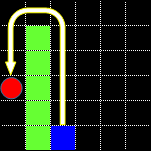
\includegraphics[width=0.5\linewidth]{Images/StaticGraphRepresentation.png}
    \caption{Nejkratší cesta od hlavy k jablku - statický graf, tělo hada - zelené čtverečky, hlava hada - modrý čtvereček, jablko - červené kolečko, šipka - nejkratší cesta od hlavy hada k jablku}
    \label{fig:StaticGraphRepresentation}
\end{figure}

Vygenerujeme si graf, kde budou propojeny všechny vrcholy tak, jak již bylo zmíněno v úvodu této kapitoly, s tím rozdílem, že do vrcholů grafu, ve kterých se nenachází tělo hada, nepovedou žádné hrany z okolních políček. Z těchto vrcholů povedou hrany pouze po směru pohybu hada do dalších částí jeho těla, tedy postupně propojíme orientovanými hranami jednotlivé části těla hada od ocasu až k hlavě. 

Tím docílíme toho, že algoritmus pro hledání nejkratší cesty se vyhne takovým cestám, ve kterých by had narazil sám do sebe. Algoritmus pro hledání nejkratší cesty tedy najde cestu podobnou jako na Obrázku~\ref{fig:StaticGraphRepresentation}. Vidíme, že nalezená cesta závisí pouze na počáteční situaci a algoritmus nebere vůbec v potaz, že se had bude hýbat (tedy, že v průběhu se může uvolnit prostor pro ještě kratší cestu).

Po vytvoření grafu algoritmus pro hledání nejkratší cesty najde nejkratší cestu s ohledem na počáteční situaci. To zároveň znamená, že pokud tělo hada momentálně zakrývá přímou cestu k jablku, tak ve statickém grafu to bude vnímáno tak, že bude cesta k jablku zakrytá pořád.

Ve hře Snake se had ovšem hýbe. Proto, pokud bude sledovat cestu nalezenou ve statickém grafu, bude ke konci obcházet překážku, která již reálně neexistuje. Při takovém přístupu budeme muset navíc po každém sebraném jablku vygenerovat nový graf, protože had neustále mění svoji pozici. Jak již bylo zmíněno, generování nového grafu je náročná operace a zejména při velkém grafu by trvala velmi dlouho. Proto statická reprezentace grafu pro simulaci hry Snake není úplně vhodná.

\section{Dynamická reprezentace}

V dynamické reprezentaci není nutné předem generovat celý graf, ale vrcholy se vytvářejí a prozkoumávají postupně během hledání nejkratší cesty. Každý vrchol obsahuje informace o svém předchozím stavu, tedy odkud jsme se do něj dostali, což umožňuje zpětně rekonstru-\\ ovat nalezenou cestu.

Tento proces probíhá iterativně – na začátku máme pouze výchozí stav (pozici hlavy hada) a postupně rozšiřujeme stavový prostor přidáváním sousedních vrcholů (možných pohybů hada). Každý nový stav odpovídá novému uspořádání herního pole po provedení daného tahu. Pokud narazíme na cílový stav (pozici jablka), můžeme zpětným sledováním předchozích stavů rekonstruovat nejkratší cestu.

Dynamická reprezentace tímto způsobem odpovídá principu prohledávání do šířky (BFS), kde se nejprve prozkoumávají všechny vrcholy v aktuální úrovni a teprve poté se přechází na další. BFS zajišťuje, že první nalezená cesta k cíli je zároveň nejkratší (pokud všechny tahy mají stejnou cenu), což je výhodné právě pro plánování pohybu hada. Hlavní rozdíl oproti statické reprezentaci je v tom, že zde nevytváříme celý graf dopředu, ale rozšiřujeme ho postupně podle potřeby. Tím se výrazně šetří paměť a umožňuje efektivní vyhledávání i ve větších prostředích. 
Podrobněji si to vysvětlíme na stejném příkladu jako při generování statického grafu (\ref{Staticky}).

\begin{figure}[h]
    \centering
    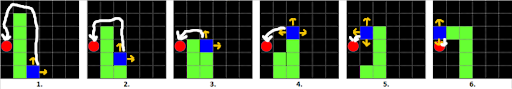
\includegraphics[width=\linewidth]{Images/DynamicGraphRepresentation.png}
    \caption{Nejkratší cesta od hlavy k jablku - dynamický graf, tělo hada - zelené čtverečky, hlava hada - modrý čtvereček, jablko - červené kolečko, žluté šipky - části grafu, které se aktuálně prozkoumávají pro hledání cesty, bílé šipky - aktuální nejkratší cesta od hlavy hada k jablku}
    \label{fig:DynamicGraphRepresentation}
\end{figure}

Máme dané pouze vrcholy reprezentující tělo hada a vrchol jablka. V prvním kroku na Obrázku~\ref{fig:DynamicGraphRepresentation} vidíme, že se had v dalším kroku dokáže pohnout pouze před sebe (rovně) nebo nahoru (doleva). To jsou vrcholy, které budeme prozkoumávat dál a také vrcholy, které vygenerujeme. Vygenerujeme je ovšem již pro situaci, která nastane, až se had na dané políčko posune. To znamená, že například pro možnost, kdy se had pohne nahoru (doleva), se každá část jeho těla posune o jedno políčko dopředu, na předcházející místo navazující části těla.

Druhý krok z Obrázku~\ref{fig:DynamicGraphRepresentation} tedy popisuje pozici hada, v případě, že se rozhodl pohnout v prvním kroku nahoru (doleva). Vidíme, že z této pozice se had může posunout buď doprava nebo nahoru (rovně). Postup z prvního kroku opakujeme a generujeme tak další možné stavy, dokud nenajdeme jablko. V každém stavu vygenerujeme pouze tělo hada a uložíme si k tomu i předchozí stav (stav, ze kterého vznikl aktuální stav).

Jak je vidět na Obrázku~\ref{fig:DynamicGraphRepresentation}, tento způsob reprezentace grafu nám umožňuje při hledání nejkratší cesty počítat i s pohybem hada v čase a díky tomu najít optimálnější cestu. Také nemusíme pokaždé, když hledáme novou cestu, vytvářet znovu celý graf, ale stačí nám vygenerovat pouze dílčí stavy, což je mnohem výhodnější nejen, co se týče paměti, ale i samotné rychlosti generování.
\chapter{Algoritmus A*}\label{A*}
Další možností, jak dohrát hru Snake, je stále hledat nejkratší možnou cestu od hlavy hada k jablku. Existuje mnoho algoritmů, kterými dokážeme najít nejkratší cestu z bodu A do bodu B, ale jedním z nejlepších je algoritmus A* (A - star). Tento algoritmus funguje na principu Dijkstrova algoritmu~\cite{Sharma2025Dijkstra}, ale ke zrychlení výpočtů využívá heuristiku. 

\section{Heuristika}
Proto abychom si lépe představili, co to heuristika je, uvedeme si příklad bludiště, kde na startu stojí myš a snaží se dostat na konec bludiště k sýru. Když se snaží myš dostat do cíle, tak může zvolit jakoukoli z možných cest. Tyto cesty mohou vést v lepším případě blíže k cíli, v horším ji zavedou naopak ještě dál od cíle, než byla na startu. Kdyby však cítila zápach sýru, věděla by vždy, jestli cítí zápach sýru méně, a tím pádem se vzdaluje, nebo jestli se zápach zesiluje a ona se k cíli naopak přibližuje (viz Obrázek~\ref{fig:MouseAndMaze}).

\begin{figure}[h]
    \centering
    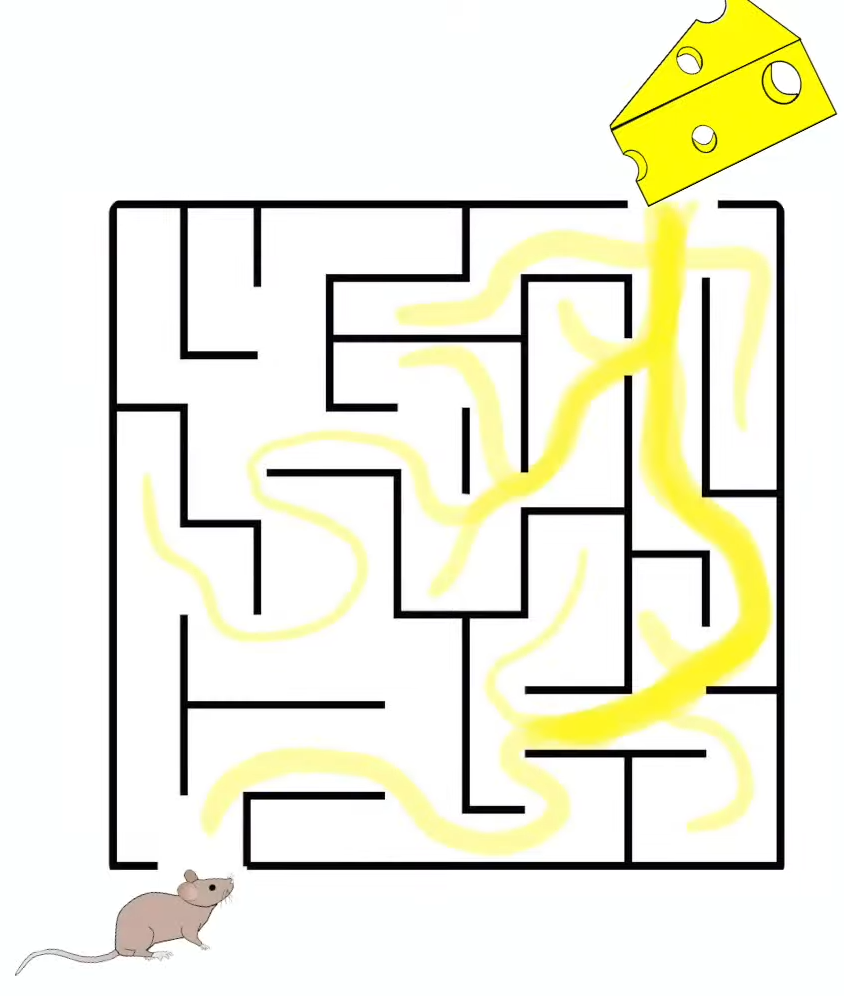
\includegraphics[width=0.5\linewidth]{Images/MouseAndMaze.png}
    \caption[Dostupné z: \url{https://www.youtube.com/watch?v=71CEj4gKDnE&ab_channel=AnishKrishnan}]{Myš a bludiště se sýrem (žluté čáry udávají intenzitu zápachu sýra)}
    \label{fig:MouseAndMaze}
\end{figure}

Díky tomu nemusí zkoušet cesty, které ji silně oddalují od cíle. Stále sice může vybrat cestu, která není správná, ale bude moci rychle rozpoznat, že tato cesta je špatná a vrátí se na tu správnou. V případě myši a sýru si můžeme heuristiku představit jako vůni, kterou myš cítí. Heuristika nám udává přibližný odhad toho, jak daleko jsme od cíle. 

V hracím poli pro hru Snake můžeme heuristiku reprezentovat jako Manhattanskou vzdále-\\nost, což je součet absolutních rozdílů souřadnic mezi dvěma body na mřížce. 

Matematicky ji lze vyjádřit jako:

\begin{center}
    \(d = |x_1 - x_2| + |y_1 - y_2|\),
\end{center}

kde (\(x_1, y_1\)) jsou souřadnice hlavy hada a (\(x_2, y_2\)) souřadnice jablka. Taková heuristika je pro náš problém vhodná, protože had se dokáže pohybovat pouze nahoru, dolů, doleva a doprava. 

\section{Popis algoritmu}

Jak již bylo zmíněno v úvodu kapitoly, algoritmus funguje na principu Dijkstrova algoritmu, má ale efektivnější výběr dalších vrcholů na zkoumání, ke kterému využívá heuristiku. V praxi se toho dosahuje prioritní frontou, ve které se vrcholy (\(V\)) řadí podle hodnoty \(f(V)\).

\(f(V)\) definujeme následně:

\begin{center}
    \(f(V) = g(V) + h(V)\),
\end{center}

kde \(g(V)\) je vzdálenost od počátečního vrcholu k mu vrcholu \(V\) a \(h(V)\) je heuristická vzdálenost od vrcholu \(V\) k cíli. 

Postup samotného algoritmu je následující (na jeho implementaci v pythonu lze nahlédnout v Ukázce kódu~\ref{lst:a_star}):

\begin{enumerate}
    \item Přidá počáteční vrchol do prioritní fronty s jeho \(f(V)\).
    \item Dokud fronta není prázdná, vrchol s nejnižší hodnotou \(f(V)\) bude z fronty vyřazen.
    \item Pokud je tento vrchol cíl, algoritmus se ukončí a vrátí zjištěnou cestu.
    \item V opačném případě se rozbalí uzel (najdou se všechny jeho sousedy) a vypočítají se \(g(V), h(V)\) a \(f(V)\) pro každého souseda. Každý soused se přidá do fronty, pokud tam ještě není, nebo pokud se k tomuto sousedovi nenajde lepší cesta.
    \item Cyklus se opakuje, dokud se nedojde k cíli nebo ve frontě už nezbyli žádné další uzly, což znamená, že neexistuje cesta od startu k vrcholu.
\end{enumerate}

\begin{figure}[H]
    \centering
    \begin{lstlisting}[language=python, style=python, caption={Implementace \(A^*\) v pythonu}, label={lst:a_star}, mathescape=true]
    def a_star(graph, start, goal):
        open_set = []
        # Push the start node with priority 0
        heapq.heappush(open_set, (0, start))
        came_from = {}
        # Cost from start to each node
        g_score = {node: float('inf') for node in graph}
        # Cost from start to start is 0
        g_score[start] = 0
        # Estimated total cost
        f_score = {node: float('inf') for node in graph}
        # Initial heuristic estimation
        f_score[start] = heuristic(start, goal)
    
        while open_set:
            # Get the node with the lowest f_score
            _, current = heapq.heappop(open_set)
            if current == goal:
                return reconstruct_path(came_from, current)
    
            for neighbor, cost in graph[current].items():
                tentative_g_score = g_score[current] + cost
                # If a better path is found
                if tentative_g_score < g_score[neighbor]:
                    came_from[neighbor] = current
                    g_score[neighbor] = tentative_g_score
                    f_score[neighbor] = g_score[neighbor] + heuristic(neighbor, goal)
                    heapq.heappush(open_set, (f_score[neighbor], neighbor))
        return None
    \end{lstlisting}
\end{figure}

\section{Nesprávnost řešení hry}

Použití algoritmu pro hledání nejkratší cesty od hlavy hada k jablku je sice z časového hlediska rozhodně rychlé, ale nikdy nedokáže zaplnit celé hrací pole, neboli úspěšně dohrát hru. Když se had bude postupně zvětšovat, bude na hracím poli méně volných políček a některá můžou být tělem hada kompletně odříznutá, kvůli čemuž had nabourá do sebe a zemře, aniž by zaplnil celé hrací pole. 

Pro objasnění si představme následující situaci. Had už je docela veliký a míří sníst další jablko. Cesta, kterou zvolil, oddělila část volných políček od ostatních. Nyní, když sní jablko a další se vygeneruje právě v tom odděleném prostoru, který v předchozích krocích vytvořil, neuvidí ho, neboli neexistuje žádná cesta od hlavy hada k jablku (viz Obrázek~\ref{fig:NoPathExistsHad}). Další případ, na kterém tento způsob kolabuje, je, když si had během pohybu k jablku odstřihne únikovou cestu, neboli cestu, po které by se mohl pohybovat zpátky poté, co jablko sní(viz Obrázek~\ref{fig:OdstrihnutiCestyHad}).

\begin{figure}[h]
    \centering
    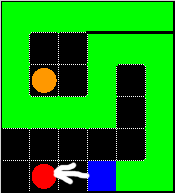
\includegraphics[width=0.4\linewidth]{Images/NoPathExistsHad.png}
    \caption{Had, který nemůže najít cestu k dalšímu vygenerovanému jablku, zelené čtverečky - tělo hada, modrý čtvereček - hlava hada, červené kolečko - jablko, které vidí aktuálně, oranžové kolečko - jablko, které uvidí poté co sebere červené jablko, bílá šipka - cesta, kterou had projde při hledání obou jablek}
    \label{fig:NoPathExistsHad}
\end{figure}

\begin{figure}[h]
    \centering
    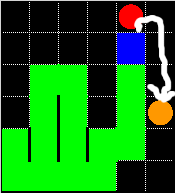
\includegraphics[width=0.4\linewidth]{Images/OdstrihnutiCestyHad.png}
    \caption{Had, který si zablokoval únikovou cestu, zelené čtverečky - tělo hada, modrý čtvereček - hlava hada, červené kolečko - jablko, které vidí aktuálně, oranžové kolečko - jablko, které uvidí poté co sebere červené jablko, bílá šipka - cesta, kterou had projde při hledání obou jablek}
    \label{fig:OdstrihnutiCestyHad}
\end{figure}
\chapter{Hamiltonovská kružnice}\label{Hamiltonovská kružnice}

Jednou z možností, jak docílit úspěšného dokončení hry Snake, je donutit hada v každé iteraci projít každé políčko právě jednou (viz Obrázek \ref{fig:Hamiltonian_cycle_example}). Takovým způsobem zamezíme tomu, že had narazí sám do sebe, a zároveň, že si had při prodlužování nezamezí úplně přístup k nějaké části hracího pole, tedy že i po maximálním prodloužení zůstane každé políčko dosažitelné. Takové cestě se v grafové teorii říká Hamiltonovská kružnice~\cite{HamiltonianCycleGFG}. Nalezení Hamiltonovské kružnice je ovšem výpočetně náročný problém (jinak známý jako problém obchodního cestujícího), konkrétně patří do třídy \(NP\)- úplných problémů. To znamená, že časová složitost nalezení Hamiltonovské kružnice je \(O(n!)\) a složitost ověření správnosti řešení je také \(O(n!)\).

\begin{figure}[!ht]
    \centering
    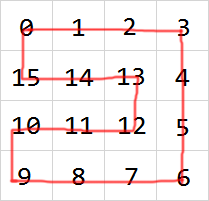
\includegraphics[width = 5cm]{Images/Hamiltonian_cycle_examle.png}
    \caption[Dostupné z: \url{https://gamedev.stackexchange.com/questions/133460/how-to-find-a-safe-path-for-an-ai-snake}]{Příklad hamiltonovské kružnice pro hrací pole \(4 \times 4\)}
    \label{fig:Hamiltonian_cycle_example}
\end{figure}

\section{Třídy složitostí}
Jedním z nejslavnějších a nejtěžších problémů, který v informatice existuje, je problém \(P\) versus \(NP\). \(P\) označuje množinu všech algoritmických problémů, které je možné vyřešit deterministickým Turingovým strojem v polynomiálním čase. Polynomem~\cite{MathTutorFunctions2025} rozumíme matematický výraz ve tvaru:
\[
P(x) = a_n x^n + a_{n-1} x^{n-1} + \cdots + a_1 x + a_0
\]
kde \(a_0, a_1, \dots, a_{n-1}, a_n\) jsou reálné koeficienty a \(n\) je nezáporné celé číslo, které určuje stupeň polynomu. Příkladem polynomu může být: \(4x^3 + 5x^2 - 8\). 

Vyřešit problém v polynomiálním čase znamená, že doba, kterou algoritmus potřebuje k vyřešení problému, je omezena polynomem závislém na velikosti vstupu. Protože Landau-\\ova~notace~\cite{BigONotationGFG} (známá také jako notace velké \(O\)) zanedbává konstantní koeficienty a zaměřu-\\je se pouze na nejvyšší prvek polynomu, můžeme říci, že algoritmus řešící problém v polynomiálním čase má časovou složitost \(O(n^k)\), kde \(n\) je velikost vstupu a \(k\) je konstanta označující stupeň polynomu. To znamená, že doba běhu algoritmu roste nejvýše polynomi-\\álně vzhledem k velikosti vstupu. To znamená, že pro dostatečně velké \(n\) je růstová rychlost takové funkce pomalejší než exponenciální \(O(2^n)\) nebo faktoriálové \(O(n!)\) složitosti, což činí problémy z třídy \(P\) prakticky řešitelnými. Pro problémy z třídy \(P\) vždy existuje řešení, které problém řeší v polynomiálním čase, a existuje i způsob, jak v polynomiálním čase ověřit správnost výsledku. 

Problémy třídy \(NP\) definujeme jako ty, které jsou v polynomiálním čase řešitelné nedeter-\\ministickým Turingovým strojem, jehož myšlenka je pouze hypotetická. Zjednodušeně můžeme říci, že \(NP\) problémy jsou takové, jejichž správnost řešení dokážeme ověřit v polynomiálním čase, ale nedokážeme přesně určit, zdali lze řešení v polynomiálním čase najít.

Všechny problémy v \(NP\) dokážeme redukovat na jiné problémy ve třídě \(NP\), to znamená, že pokud bychom dokázali najít řešení v polynomiálním čase pro jeden problém z \(NP\), dokázali bychom tím, že všechny problémy v \(NP\) lze řešit v polynomiálním čase. To by ale také znamenalo, že \(P = NP\). Většina odborníků se ovšem domnívá, že takový efektivní algoritmus neexistuje, a proto je většina přesvědčena o tom, že rovnost neplatí, tedy že  $P \neq NP$.

Třídy složitosti můžeme dále dělit na \(NP\)- úplné a na \(NP\)- těžké problémy~\cite{demaine2016complexity}. \(NP\)- těžké problémy popisují třídu, ve které jsou problémy těžké alespoň jako všechny \(NP\) složité problémy. To znamená, že bude obsahovat problémy, které budou určitě těžší než \(NP\). Třída \(NP\)- úplných problémů obsahuje úlohy, které jsou určitě těžké jako všechny \(NP\) problémy, ale nejsou těžší. To znamená, že tato třída leží přímo mezi \(NP\) a \(NP\)- těžkých problémů (hierarchie tříd je zobrazena na Obrázku~\ref{fig:HierarchieProblemTrid}).

\begin{figure}[!ht]
    \centering
    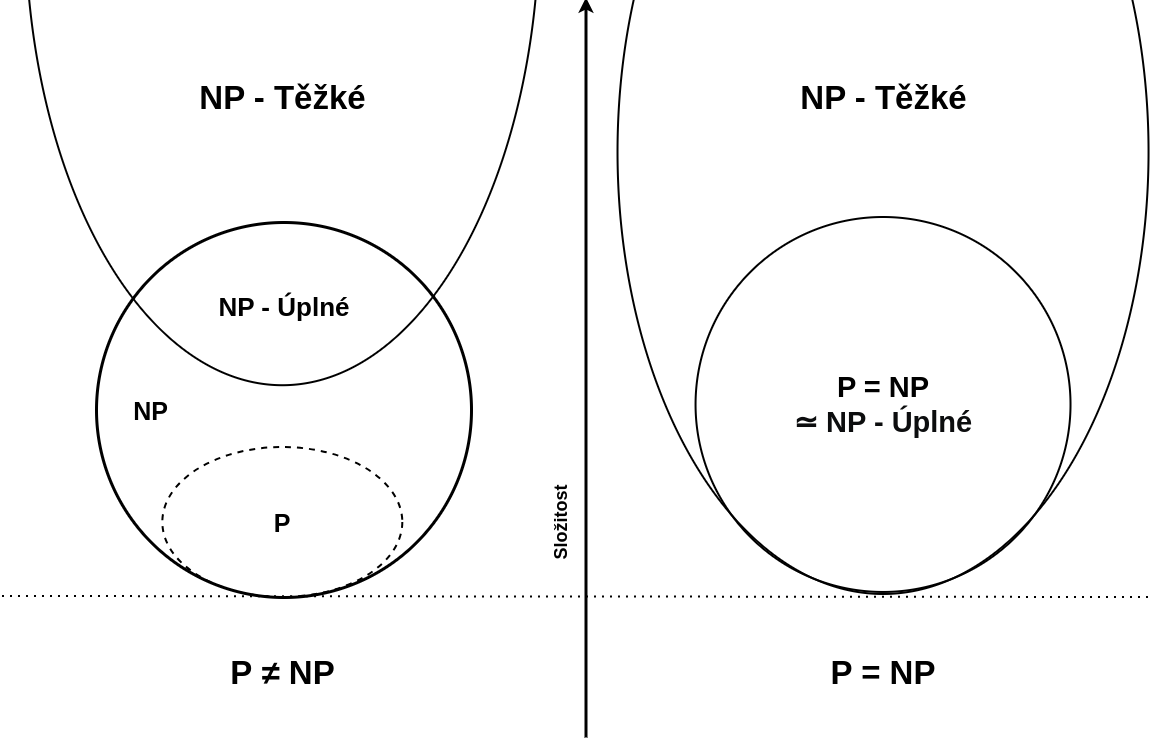
\includegraphics[width = 12cm]{Images/HierarchieProblemTrid.png}
    \caption{Hierarchie tříd složitosti}
    \label{fig:HierarchieProblemTrid}
\end{figure}

\section{Neúplné řešení}
Jak bylo řečeno dříve, hledání Hamiltonovské kružnice patří mezi \(NP\)- úplné problémy, tedy že pro obecný graf neumíme najít Hamiltonovskou kružnici efektivně. Jsme schopni nalézt takovou kružnici v časové složitosti \(O(n!)\), to znamená, že pro velmi malá \(n\) dokáže-\\me najít kružnici celkem rychle, ale třeba už pro \(n = 17\) by výpočet trval přibližně 4 dny. 

Graf používaný ve hře Snake je čtvercový. Omezení daná z jeho definice nám usnadní úlohu hledání kružnice, protože problém již nemusíme řešit pro obecný graf, který má mnohem více hran. Pro čtvercový graf jde relativně snadno najít Hamiltonovská kružnice, pomocí algoritmu od Johna Tapsella~\cite{tapsell2025snake}.

\subsection{Algoritmus poloviční kostry grafu}

Nejdůležitější myšlenka algoritmu pro hledání Hamiltonovské kružnice ve čtvercovém grafu se zakládá na kostře grafu (Obrázek~\ref{fig:SpanningTreeSmallerGraph}). Pokud se pozorně podíváme na kostru nějakého čtvercového grafu, zjistíme, že obvod kostry je vlastně Hamiltonovská kružnice pro graf dvakrát větší (Obrázek~\ref{fig:SpanningTreeToHamilton}). To znamená, že pro nalezení kružnice potřebujeme vygenerovat kostru pro graf s dvakrát menšími rozměry než má graf, ve kterém se snažíme najít kružnici. 

\begin{figure}[!ht]
    \centering
    \begin{subfigure}[t]{0.45\textwidth}
        \centering
        
\includegraphics[width=\textwidth]{Images/SpanningTreeSmallerGraph.png}
        \caption{Kostry grafu}
        \label{fig:SpanningTreeSmallerGraph}
    \end{subfigure}
    \hfill
    \begin{subfigure}[t]{0.45\textwidth}
        \centering
        
\includegraphics[width=\textwidth]{Images/SpanningTreeToHamilton.png}
        \caption{Transformace z kostry na Hamiltonovskou kružnici}
        \label{fig:SpanningTreeToHamilton}
    \end{subfigure}
    \caption[Dostupné z: \url{https://miro.medium.com/v2/resize:fit:600/format:webp/1*kviW8mFsjXoLeOTdqTmbmA.png} \textbf{,}  \url{https://miro.medium.com/v2/resize:fit:600/format:webp/1*aB8mFapIsycDGVueoSpr1Q.png}]{Kostry grafu a jejich transformace}
\end{figure}

Nalezení kostry velmi ulehčuje hledání Hamiltonovské kružnice ve čtvercovém grafu, ale bohužel můžeme tímto způsobem vygenerovat pouze podmnožinu všech možných Hamiltonovských kružnic (Obrázek~\ref{fig:NotAllGenerations}). Zvětšováním rozměrů grafu \(n \times m\), ve kterém hledáme kostru, se zároveň omezuje i velikost grafu, ve kterém následně hledáme Hamilto-\\novskou kružnici – ta je určena rozměry \(2n \times 2m\).

Pro úspěšné vyřešení hry Snake ovšem nepotřebujeme najít všechny možné Hamiltonovské kružnice, stačí nám alespoň jedna. Proto můžeme přístup založený na hledání kostry grafu bez obav využít.

\begin{figure}[!t]
    \centering
    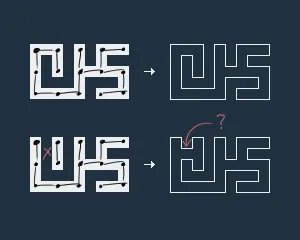
\includegraphics[width = 0.8\textwidth]{Images/NotAllGenerations.png}
    \caption[Dostupné z: \url{https://miro.medium.com/v2/resize:fit:600/format:webp/1*P8932ZvcHs8vOl3OXzJCnA.png}]{Kostra grafu, která neumožňuje vygenerovat všechny možné Hamiltonovské kružnice, ale pouze jejich podmnožinu}
    \label{fig:NotAllGenerations}
\end{figure}

\subsection{Nález Hamiltonovské kružnice}

Díky algoritmu popsanému v předchozí sekci dokážeme snadno najít Hamiltonovskou kružnici, jako obvod kostry dvakrát menšího grafu. Jak ale v praxi vytvoříme graf jako obvod kostry? 

První, co si musíme uvědomit, je, že každý vrchol z menšího grafu má okolo sebe vždy čtyři vrcholy většího grafu. Ke každému vrcholu musíme tedy správně přiřadit čtyři vrcholy většího grafu. Zkusme přemýšlet nad konkrétním příkladem.

Graf, ve kterém budeme hledat kostru, bude mít rozměry \(3 \times 3\), tím pádem graf, ve kterém se budeme snažit najít kružnici, má rozměry \(6 \times 6\). Vrcholy budeme číslovat od nuly, menší graf bude mít vrcholy 0-8, větší graf 0-35. Z Obrázku~\ref{fig:HledaniKruzniceZKostry} je patrné, že stačí zjistit číslo vrcholu, který je od vrcholu menšího grafu umístěn vlevo nahoře, protože ostatní tři vrcholy dokážeme zjistit přičtením fixních konstant. Jak se konkrétně přiřadí sousední vrcholy, ilustrujeme pomocí metody \texttt{neighbor\_nodes}~\ref{lst:neighbor_nodes}. 

Když už máme přiřazené sousední vrcholy, stačí zjistit, které z nich potřebujeme spojit, abychom získali Hamiltonovskou kružnici. Z Obrázku~\ref{fig:HledaniKruzniceZKostry} vidíme, že rozhodně můžeme vždy spojit vrcholy, které se nacházejí v rohu hracího pole (v našem případě $[6, 0]$ a $[0, 1]$, nebo $[24, 30]$ a $[30, 31]$ atd.). Další hrany, o kterých určitě víme, že je můžeme vytvořit, jsou hrany mezi vrcholy, které se nacházejí na krajích hracího pole a zároveň sousedí s vrcholy přiřazenými ke stejnému vrcholu z menšího grafu. To jsou např.: $[12, 18]$, $[2, 3]$ nebo $[17, 23]$.

\begin{figure}[H]
    \centering
    \begin{lstlisting}[language=python, style=python, caption={Určení sousedních vrcholů většího grafu}, label={lst:neighbor_nodes}, mathescape=true]
    def neighbor_nodes(self):
        nodes_for_smaller_nodes = {}
        for x in range(self.vertices):
            left_up = ((x // self.number_of_nodes_on_side) 
            * 4 * self.number_of_nodes_on_side)
            + ((x % self.number_of_nodes_on_side) * 2)
            right_up = left_up + 1
            left_down = left_up + (self.number_of_nodes_on_side * 2)
            right_down = left_down + 1
            # Save neighbor nodes into the dictionary
            nodes_for_smaller_nodes[x] = {
                "left_up": left_up,
                "right_up": right_up,
                "left_down": left_down,
                "right_down": right_down
            }
        return nodes_for_smaller_nodes
    \end{lstlisting}
\end{figure}

O ostatních hranách již nemůžeme rozhodnout tak jednoduše bez využití kostry menšího grafu. Vezměme tedy např. hranu z menšího grafu $[0, 1]$, vidíme, že pokud chceme utvořit obrys této hrany, potřebujeme spojit vrcholy nad hranou $[1, 2]$ a pod hranou $[7, 8]$. Tyto hrany jsou rovnoběžné k hraně $[0, 1]$ malého grafu. Kdyby hrana $[0, 1]$ mezi vrcholy malého grafu nebyla, museli bychom spojit sousední vrcholy bodů 0 a 1 ve směru kolmém na hypotetickou hranu $[0, 1]$. To znamená hrany $[1, 7]$ a $[2, 8]$. Takovým způsobem pokračujeme ve stavbě celého grafu. Procházíme všechny vrcholy malého grafu, které tvoří kostru. Pokud existuje hrana mezi dvěma vrcholy v menším grafu, spojíme odpovídající sousední vrcholy v rozšířeném grafu rovnoběžně se směrem této hrany. Pokud v menším grafu hrana neexistuje, spojíme odpovídající sousední vrcholy ve větším grafu ve směru kolmém na směr, ve kterém by tato hrana vedla.

\begin{figure}[H]
    \centering
    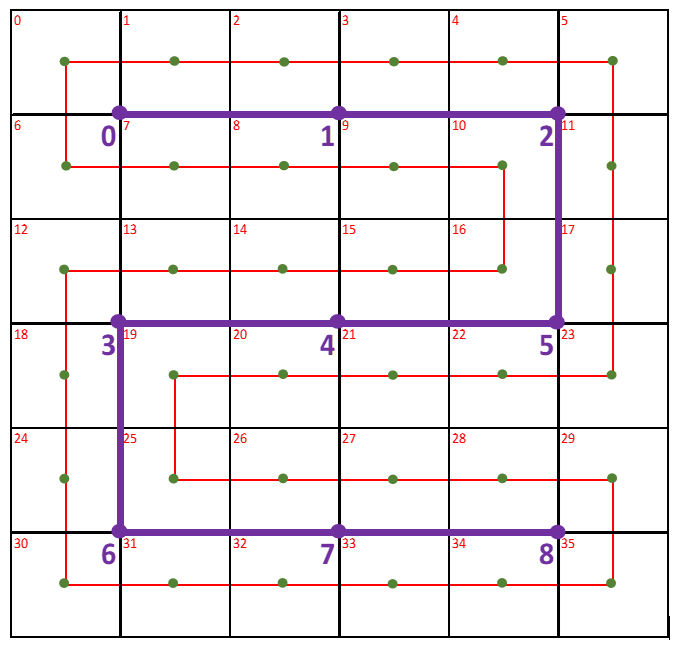
\includegraphics[width=0.7\linewidth]{Images/HledaniKruzniceZKostry.png}
    \caption{Kostra malého grafu, Hamiltonovská kružnice velkého grafu, sousední vrcholy (zelené)}
    \label{fig:HledaniKruzniceZKostry}
\end{figure}

\section{Rychlost řešení hry}

Použití Hamiltonovské kružnice pro úspěšné dokončení hry Snake funguje vždy~\cite{Graafsma2025Snake}. V porovnání s jinými metodami, které budou popsány dále v textu, je ovšem nesmírně pomalé (porovnání v kapitole~\ref{Srovnání algoritmů}). Cílem této práce nebylo pouze úspěšné dokončení hry, ale její dokončení v co nejkratším čase.

Při tomto přístupu k řešení hry se například vůbec neuvažuje nad tím, kde se objeví další jablko. To znamená, že na začátku hry, kdy je had ještě velmi malý, je průměrná vzdálenost, kterou had musí urazit k jablku, polovina hracího pole, neboli  \(\frac{n}{2}\) všech vrcholů v grafu. V polovině hry, kdy had zabírá nějaký prostor, se už jablko musí objevit blíže k hadovi a na konci hry, když had zabírá skoro celé hrací pole, se bude jablko objevovat přímo před ním. K poslednímu jablku, které had sebere, urazí cestu dlouhou jedno políčko.

Tím pádem dokážeme vypočítat průměrný počet tahů na hru při použití Hamiltonovské kružnice pro dokončení hry. Počet tahů vyjádříme následujícím vztahem: 
\begin{center}
    $\frac{\frac{n}{2} \cdot n}{2}$
\end{center}
kde \(n\) je počet vrcholů v grafu (počet políček v herním poli)~\cite{alphaphoenix2020snake}.  Na závislost můžeme nahlédnout také na Obrázku~\ref{fig:HamiltonianCycleDuration}.

\begin{figure}
    \centering
    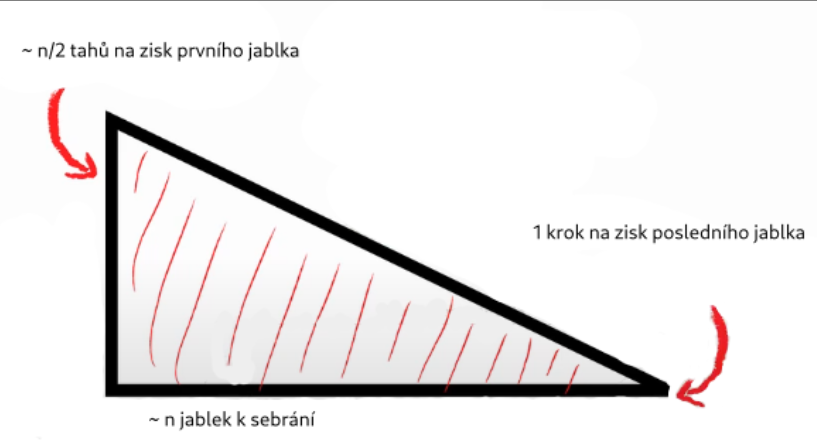
\includegraphics[width=0.7\linewidth]{Images/HamiltonianCycleDuration.png}
    \caption[Dostupné z: \url{https://www.youtube.com/watch?v=TOpBcfbAgPg&t=245s&ab_channel=AlphaPhoenix}]{Výpočet přibližného počtu tahů}
    \label{fig:HamiltonianCycleDuration}
\end{figure}
\chapter{Řešení}\label{Řešení}
V kapitolách~\ref{Hamiltonovská kružnice} a~\ref{A*} jsme uvedli možné přístupy použitelné pro simulaci hry Snake a k dosažení jejího dokončení. Oba přístupy ale mají své nedostatky. V této kapitole vysvětlím své optimálnější řešení problému, ke kterému jsem využil algoritmus Johna Tapsella~\cite{tapsell2025snake}.

\section{Popis algoritmu}

Algoritmus využívá Hamiltonovské kružnice, protože jak již víme, sledováním takové kružnice umožníme hadovi hru úspěšně dohrát, aniž by v průběhu narazil sám do sebe. Po vygenerování kružnice jí stále budeme následovat, ale s tím rozdílem, že si občas cestu zkrátíme, abychom sebrali jablko rychleji a následně se opět vrátili na kružnici. Tím bychom dokázali hru ve fázi, kdy je had ještě krátký, výrazně urychlit. 

Na příkladu si uveďme, jak přesně bychom museli zkratky vytvářet. Na Obrázku ~\ref{fig:HadZkratkyReseni} vidíme, že had se nachází na políčkách 13, 14 a na políčku 15 je hlava hada. Jablko se nachází na políčku 21. Místo toho, abychom následovali další 4 políčka po kružnici, můžeme udělat zkratku z políčka 15 na políčko 20 a následně se přemístit na políčko 21 a sebrat jablko. Tím ušetříme čtyři tahy. 

Zkratky můžeme vytvářet pouze po směru Hamiltonovské kružnice. To znamená, že např. z vrcholu 26 bychom dokázali vytvořit zkratku do vrcholu 35, ale z vrcholu 16 bychom nemohli utvořit zkratku na vrchol 9. Tím docílíme toho, že hlava hada nikdy nepředběhne jeho ocas. 

Dále potřebujeme kontrolovat, jestli má had dostatek prostoru pro růst po sebrání jablka, při využití zkratky. Protože pokud využije zkratku a přitom nemá dostatek prostoru na růst dále ve směru kružnice, poroste do sebe a tím pádem sám do sebe narazí a zemře.

V praxi to funguje tak, že pokaždé, když had sebere jablko, najdeme nejkratší cestu k dalšímu jablku a ověříme, jestli zkratka daná touto nejkratší cestou vyhovuje všem námi dříve stanoveným podmínkám. Pokud ano, had využije zkratku, pokud ne, pokračuje ve sledování kružnice.

\begin{figure}[H]
    \centering
    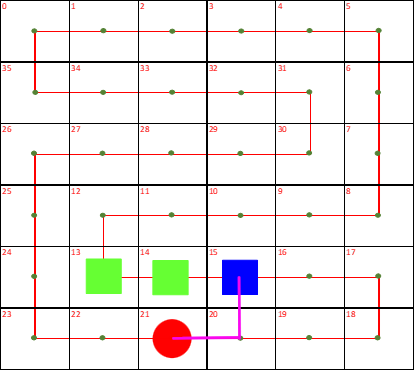
\includegraphics[width=0.8\linewidth]{Images/HadZkratkyReseni.png}
    \caption{Had následující Hamiltonovskou kružnici, zelené čtverečky - tělo hada, modré čtverečky - hlava hada, červené kolečko - jablko, růžová lomená čára - zkratka, kterou had udělá}
    \label{fig:HadZkratkyReseni}
\end{figure}

\section{Implementace algoritmu}

Vyhovující zkratky budeme generovat pomocí jemně upraveného A* algoritmu. Tedy po-\\každé, když had sebere jablko, pomocí upraveného algoritmu A* najdeme nejkratší cestu od hlavy hada k jablku a vyhodnotíme, zda nalezenou zkratku použijeme, nebo ne.

Aby se nalezena cesta dala považovat za zkratku, musí obsahovat pouze takové vrcholy, které jsou vzestupně seřazeny podle pozice v Hamiltonovské kružnici. Například, pokud se jablko nachází na políčku 30 a had se nachází na pozicích 13, 14 a 15 (hlava hada), had nemůže využít zkratku, která by vedla z 15 do 10, pak do 29 a potom by následoval za jablkem do pole 30. Taková cesta nesplňuje výše zmíněné seřazení vrcholů. Nejlepší cesta, kterou může využít, obsahuje zkratku z políčka 15 do 20 a poté následovat Hamiltonovskou kružnici až k jablku (viz Obrázek~\ref{fig:HadZkratkyPrikladyReseni}).

\begin{figure}[h]
    \centering
    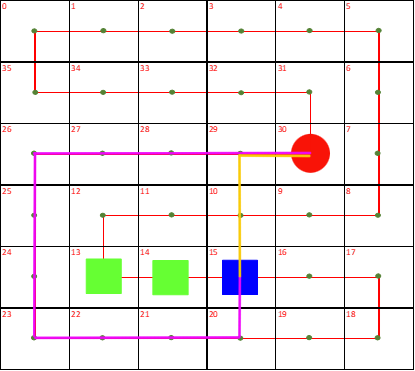
\includegraphics[width=0.8\linewidth]{Images/HadZkratkyPrikladyReseni.png}
    \caption{Had následující Hamiltonovskou kružnici, zelené čtverečky - tělo hada, modré čtverečky - hlava hada, červené kolečko - jablko, růžová lomená čára - zkratka, kterou had může udělat, žlutá lomená čára - zkratka, kterou had nemůže udělat}
    \label{fig:HadZkratkyPrikladyReseni}
\end{figure}

Modifikovaná verze algoritmu A* (implementace algoritmu v jazyce Python k nahlédnutí v Ukázce kódu~\ref{lst:a_star_modification}) povoluje vybrat do cesty pouze ty vrcholy, které jdou vzestupně podle Hamiltonovské kružnice.

\begin{figure}[H]
    \centering
    \begin{lstlisting}[language=python, style=python, caption={Modifikovaný A*}, label={lst:a_star_modification}, mathescape=true]
    def a_star(game_state: GameState, a_pos: tuple[int, int], n_rows: int, n_cols: int, ham):
     open_set = []
     # Push the initial state with priority 0
     heapq.heappush(open_set, PrioritizedItem(0, game_state))
         # Iterate over neighboring nodes
         for neighbor in current.neighbors(n_rows, n_cols):
             tentative_g_score = g_score[current.h_pos] + 1
             neighbor.predecessor = current

             # Convert game coordinates to graph representation
             s_h_pos = game_to_graph(current.h_pos, n_cols)
             e_h_pos = game_to_graph(neighbor.head_position, n_cols)
             
             # Check if the neighbor has a lower cost path or is unvisited
             if neighbor.h_pos not in g_score or tentative_g_score < g_score[neighbor.h_pos]:
                 # Ensure movement follows Hamiltonian cycle constraints
                 if ham[s_h_pos] <= ham[e_h_pos] or (ham[s_h_pos] == (n_cols * n_cols)-1 and ham[e_h_pos] == 0):
                     g_score[neighbor.h_pos] = tentative_g_score
                     f_score[neighbor.h_pos] = tentative_g_score + heuristic(neighbor.h_pos,a_pos)
                     neighbor.predecessor = current
                     
                     # Add neighbor to open set if it's not already included
                     if neighbor not in [item.state for item in open_set]:
                         heapq.heappush(open_set, PrioritizedItem(f_score[neighbor.h_pos], neighbor))
        return None
    \end{lstlisting}
\end{figure}
\chapter{Srovnání algoritmů}\label{Srovnání algoritmů}

V této kapitole provedeme srovnání jednotlivých přístupů k řešení hry Snake. Zaměříme se na dvě hlavní kritéria: úspěšnost dokončení hry a efektivitu. Přičemž úspěšností myslíme, jak často algoritmus vede k vítězství - zaplnění celé hrací plochy bez kolize. Efektivitou rozumíme, jak rychle had sbírá jablka a jak plynule se pohybuje bez zbytečných tahů.

Porovnáme tři přístupy na herním poli \(10 \times 10\). Maximální dosažitelné skóre je 97. Prvním je A* (viz Kapitola~\ref{A*}), heuristický algoritmus hledající nejkratší cestu od hlavy hada k jablku. Další je Hamiltonovská kružnice (viz Kapitola~\ref{Hamiltonovská kružnice}), která představuje předem vygenerovanou cestu, jež zajišťuje, že had nikdy nenarazí sám do sebe. Posledním je algorit-\\mus zkratek (viz Kapitola~\ref{Řešení}), který kombinuje Hamiltonovskou kružnici s možností vytvářet optimalizované zkratky pomocí algoritmu A*.

\section{Výsledky A*}

Řešení problému s využitím algoritmu A*, který hledá nejkratší cestu od hlavy hada k jablku, nedopadlo nikdy úspěšně. Had z více než 300 pokusů ani jednou nedohrál hru (nezaplnil celou hrací plochu bez kolize). Průměrná délka hry trvala 21 sekund. Had v průměru dosáhl skóre 28 a průměrný počet tahů byl 223. Na Grafu~\ref{fig:Počet tahů - A_} můžeme vidět četnosti tahů během různých her. Vidíme, že modus počtů tahů je 161-194. V grafu~\ref{fig:Skóre _ Tahy - A_} je znázorněna závislost skóre na počtu tahů. Vidíme, že čím více tahů had udělal, tím většího skóre dosáhl.

\begin{figure}[H]
    \centering
    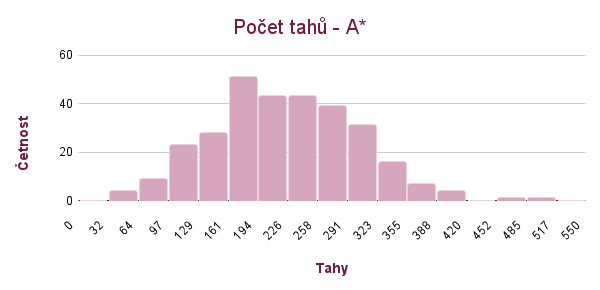
\includegraphics[width=\linewidth]{Images/Počet tahů - A_.png}
    \caption{Četnost tahů během různých her - A*}
    \label{fig:Počet tahů - A_}
\end{figure}

\begin{figure}[H]
    \centering
    \includegraphics[width=\linewidth]{Images/Skóre _ Tahy - A_.png}
    \caption{Závislost skóre na počtu tahů - A*}
    \label{fig:Skóre _ Tahy - A_}
\end{figure}

\section{Hamiltonovská kružnice}

Využití sledování Hamiltonovské kružnice k řešení problému bylo \(100\%\) úspěšné. Průměrná délka hry z 200 pokusů byla 4 minuty a 21 sekund a průměrný počet tahů, který závisí na pozicích generovaných jablek, byl 2485. Největší počet tahů, kterého bylo dosaženo, je 2997 a nejmenší počet tahů byl 1921. V Grafu~\ref{fig:Počet tahů - Hamiltonovská kružnice} je znázorněna četnost tahů během různých her. Je zcela zřejmé, že modus počtů tahů ve hře je 2357-2464.

\begin{figure}[H]
    \centering
    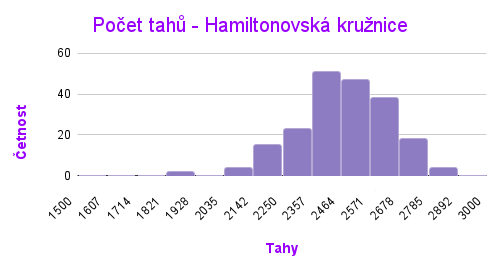
\includegraphics[width=\linewidth]{Images/Počet tahů - Hamiltonovská kružnice.png}
    \caption{Četnost tahů během různých her - Hamiltonovská kružnice}
    \label{fig:Počet tahů - Hamiltonovská kružnice}
\end{figure}

\section{Algoritmus zkratek}

Algoritmus, který vytváří zkratky v existující Hamiltonovské kružnici, vedl v \(72\%\) přípa-\\dech z přibližně 230 pokusů k úspěšnému dokončení hry. V těchto úspěšných pokusech byla průměrná délka hry 3 minuty a 2 sekundy. Průměrný počet tahů, v úspěšných hrách, byl 1825. V Grafu~\ref{fig:Počet tahů - Algoritmus zkratek} je vidět četnost tahů během úspěšných her. Modusy počtů tahů, provedených během hry, jsou 1722-1833 a 1833-1944. Největší počet tahů za jednu hru byl 2112. Tak vysoký počet naznačuje, že had v průběhu hry nevyužil skoro žádné zkratky, protože se počet tahů blíží jednomu z nejmenších počtů tahů, při prostém využití Hamilto-\\novské kružnice. V Grafu~\ref{fig:Tahy _ čas - Algoritmus zkratek} je, z pouze úspěšných pokusů, zobrazena závislost počtu tahů na čase.

\begin{figure}[H]
    \centering
    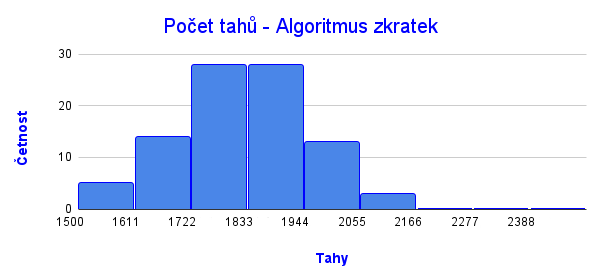
\includegraphics[width=\linewidth]{Images/Počet tahů - Algoritmus zkratek.png}
    \caption{Četnost tahů během různých her - Algoritmus zkratek}
    \label{fig:Počet tahů - Algoritmus zkratek}
\end{figure}

\begin{figure}[H]
    \centering
    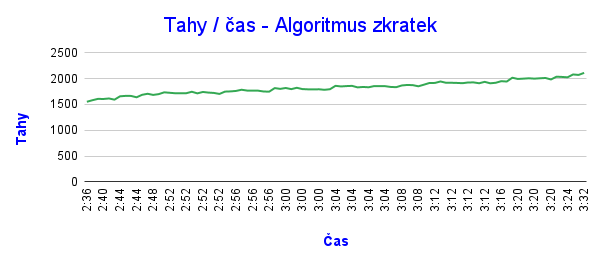
\includegraphics[width=\linewidth]{Images/Tahy _ čas - Algoritmus zkratek.png}
    \caption{Závislost počtu tahů na čase - Algoritmus zkratek}
    \label{fig:Tahy _ čas - Algoritmus zkratek}
\end{figure}

\section{Vzájemné porovnání jednotlivých přístupů}
Pomocí tabulky~\ref{table:PorovnaniPristupu} si porovnáme jednotlivé přístupy. Můžeme vidět, že algoritmus \(A*\), kvůli tomu, že hru nikdy nedokončil, má ve všech měřených oblastech velmi odlišné hodnoty, proto budeme srovnávat spíše algoritmus zkratek a Hamiltonovskou kružnici. Hamiltonovská kružnice byla v dokončení hry \(100\%\) úspěšná, na rozdíl od algoritmu zkratek, který byl úspěšný pouze ze \(72\%\). Průměrná délka úspěšné hry algoritmu zkratek byla 3 minuty a 2 sekundy, což je přibližně o \(30\%\) lepší čas, než u prostého sledování Hamiltonovské kružnice. Průměrný počet tahů, v úspěšných hrách algoritmu zkratek, byl 1825 a to je skoro o 100 tahů méně, než nejmenší počet tahů při využití pouze Hamiltonovské kružnice. Modusy tahů v úspěšných hrách algoritmu zkratek jsou výrazně menší než modus tahů na hru u Hamiltonovské kružnice. 

\begin{table}[h!]
\centering
\begin{tabular}{ | p{4,5cm} || p{1,7cm} | p{2cm} | p{2cm} | p{2cm} |  }
 \hline
 Algoritmus & Úspěšnost v \% & Průměrný čas hry & Průměrný počet tahů na hru & Modus tahů na hru \\
 \hline
 A*  & 0 & 21 s & 223 & 194 \\
 Hamiltonovská kružnice & 100 & 4 min 21 s & 2485 & 2357-2464 \\
 Algoritmus zkratek & 72 & 3 min 2 s & 1825 & 1722-1833, 1833-1944 \\
 \hline
\end{tabular}
\caption{Porovnání jednotlivých přístupů k řešení hry Snake. Porovnáváme úspěšnost dokončení hry, průměrný čas pro dokončení hry, průměrný a nejčetnější počet tahů na hru pro algoritmy A*, Hamiltonovskou kružnici a algoritmus zkratek.}
\label{table:PorovnaniPristupu}
\end{table}

Tato zjištění ukazují, že i když Hamiltonovská kružnice garantuje \(100\%\) úspěšnost, algorit-\\mus zkratek je efektivnější, pokud jde o rychlost dokončení hry a počet tahů. Algoritmus zkratek poskytuje rychlejší a plynulejší hru s nižším počtem tahů, což jej činí nejefektivněj-\\ším přístupem mezi těmito třemi algoritmy pro řešení hry Snake.
\chapter{Závěr}

V této práci jsem analyzoval a porovnal tři různé algoritmy pro řešení hry Snake: A*, Hamiltonovskou kružnici a algoritmus zkratek. Hodnotil jsem je z hlediska úspěšnosti dokončení hry a efektivity sbírání jablek. Při testování jsem zjistil, že samotný algoritmus A* nebyl nikdy úspěšný, protože had se dříve či později dostal do situace, kdy narazil do sebe. Ačkoliv A* efektivně hledal nejkratší cestu k jablku, nebyl schopen zajistit dlouhodo-\\ bě bezpečný pohyb hada.

Hamiltonovská kružnice se ukázala jako stoprocentně spolehlivá strategie, která vždy vedla k úspěšnému dokončení hry. Jejím hlavním nedostatkem však byla nízká efektivita – had často prováděl zbytečně dlouhé tahy, což značně prodlužovalo dobu trvání hry.

Nejlepším kompromisem se ukázal být algoritmus zkratek, který kombinuje Hamiltonov-\\skou kružnici s možností vytvářet optimalizované cesty pomocí modifikovaného algoritmu A*. Tento přístup vedl k dokončení hry v přibližně \(72\%\) případech a zároveň výrazně zkrátil počet tahů i celkovou dobu hry v porovnání s čistým následováním Hamiltonovské kružnice.

Při implementaci jsem narazil na několik zásadních problémů. Nejnáročnější bylo nalezení Hamiltonovské kružnice pro dané herní pole. Tento problém patří mezi \(NP\)-úplné problé-\\my, což znamená, že neexistuje efektivní algoritmus pro jeho řešení v obecném případě. Musel jsem proto využít speciální postupy pro nalezení kružnice. Dalším problémem byla efektivní detekce možných zkratek, která musela respektovat pořadí vrcholů v Hamiltonov-\\ské kružnici. 

Nakonec se mi podařilo vytvořit funkční a relativně efektivní řešení, přesto stále vidím prostor pro další zlepšení. Možným rozvojem projektu by bylo například dynamické upra-\\vování Hamiltonovské kružnice podle aktuální situace na herním poli nebo využití pokroči-\\lejších heuristik pro rozhodování o použití zkratek.

Celkově hodnotím projekt jako úspěšný, protože se mi podařilo implementovat a otestovat různé strategie řízení hada, porovnat jejich výkonnost a identifikovat nejefektivnější přístup. Zároveň jsem získal cenné zkušenosti s algoritmy pro hledání cest a jejich aplikací na problém s dynamickým prostředím.


\newpage
\begingroup
\let\clearpage\relax
\renewcommand{\listfigurename}{Seznam ukázek obrázků}
\listoffigures
\endgroup


\newpage
\begingroup
\let\clearpage\relax
\renewcommand{\lstlistlistingname}{Seznam ukázek kódu}
\lstlistoflistings
\endgroup

\renewcommand{\bibname}{Seznam zdrojů}
\printbibliography

\end{document}